\documentclass{article}

\usepackage[utf8]{inputenc}
\usepackage[spanish]{babel}
\usepackage{listingsutf8}
\usepackage{xcolor}
\usepackage{pdfpages}
\usepackage{geometry}
% to install algorithm2e pckg: sudo apt-get install texlive-science
\usepackage[ruled, vlined, nofillcomment]{algorithm2e}
\usepackage{float}
%\usepackage{hyperref}
\usepackage{amsmath}
\usepackage{framed}
\usepackage{enumitem}

\geometry{
    a4paper,
    margin=1.2in
}

% Some settings for coding style
\lstset{
    basicstyle=\linespread{0.9}\ttfamily\footnotesize,
    frame=single,
    frameround=tttt,
    numbers=left,
    numberstyle=\tiny,
    linewidth=14cm,
    literate=
      {á}{{\'a}}1 {é}{{\'e}}1 {í}{{\'i}}1 {ó}{{\'o}}1 {ú}{{\'u}}1
      {Á}{{\'A}}1 {É}{{\'E}}1 {Í}{{\'I}}1 {Ó}{{\'O}}1 {Ú}{{\'U}}1
      {à}{{\`a}}1 {è}{{\`e}}1 {ì}{{\`i}}1 {ò}{{\`o}}1 {ù}{{\`u}}1
      {À}{{\`A}}1 {È}{{\'E}}1 {Ì}{{\`I}}1 {Ò}{{\`O}}1 {Ù}{{\`U}}1
      {ä}{{\"a}}1 {ë}{{\"e}}1 {ï}{{\"i}}1 {ö}{{\"o}}1 {ü}{{\"u}}1
      {Ä}{{\"A}}1 {Ë}{{\"E}}1 {Ï}{{\"I}}1 {Ö}{{\"O}}1 {Ü}{{\"U}}1
      {â}{{\^a}}1 {ê}{{\^e}}1 {î}{{\^i}}1 {ô}{{\^o}}1 {û}{{\^u}}1
      {Â}{{\^A}}1 {Ê}{{\^E}}1 {Î}{{\^I}}1 {Ô}{{\^O}}1 {Û}{{\^U}}1
      {œ}{{\oe}}1 {Œ}{{\OE}}1 {æ}{{\ae}}1 {Æ}{{\AE}}1 {ß}{{\ss}}1
      {ű}{{\H{u}}}1 {Ű}{{\H{U}}}1 {ő}{{\H{o}}}1 {Ő}{{\H{O}}}1
      {ç}{{\c c}}1 {Ç}{{\c C}}1 {ø}{{\o}}1 {å}{{\r a}}1 {Å}{{\r A}}1
      {€}{{\euro}}1 {£}{{\pounds}}1 {«}{{\guillemotleft}}1
      {»}{{\guillemotright}}1 {ñ}{{\~n}}1 {Ñ}{{\~N}}1 {¿}{{?`}}1
}

\title{66.26 - Arquitecturas Paralelas\\Trabajo final}

\author{
    \\\\\\\\
%     \Large{Group name}\\
    Arturi, Augusto(\texttt{\#97498})\\\texttt{turitoh@gmail.com}\\
    \\
    Rozanec, Matias (\texttt{\#97404})\\\texttt{rozanecm@gmail.com}\\
%    \\
%    surname2, name2 (\texttt{\#padron})\\\texttt{mail@example.com}\\
    \\\\\\\\\\\\\\
}

\date{Diciembre 2018}

\begin{document}
\maketitle
\begin{figure}[!htp]
    \centering
    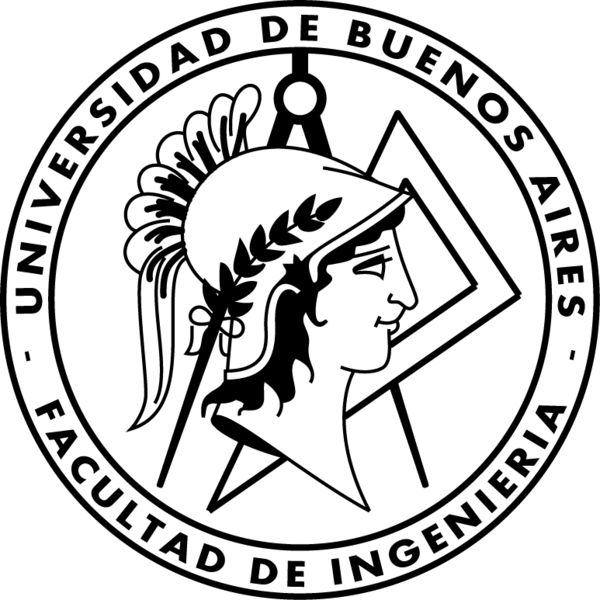
\includegraphics[scale=1]{../res/fiuba_logo.png} 
\end{figure}
\begin{center}\normalsize{Facultad de Ingeniería, Universidad de Buenos Aires}\end{center}
\newpage

\tableofcontents
\newpage

% *** CONSIGNA ***
% \part{Consigna}
% \includepdf[pages=-]{consigna.pdf}

% *** RESOLUCION ***

\part{Introducción}

La Dinámica de Fluidos (CFD por sus siglas en inglés) se usa para simular el flujo de fluidos en aplicaciones industriales. A medida que los simuladores se vuelven más complejos, el poder de cálculo que se requiere aumenta significativamente. En casos en que el tiempo de cómputo puede llevar días o meses, aún cambios relativamente pequeños en la eficiencia de cálculo pueden representar grandes mejoras en el cómputo.

El código usado para correr las simulaciones es OpenFOAM, un paquete CFD open source. Este software es diseñado para correr en paralelo, pudiendo ser configurado para correr efectivamente en cualquier cantidad de cores distribuidos a lo largo de cualquier número de computadoras presentes en una misma red. Idealmente los casos que se puedan correr en paralelo serán divididos en partes iguales distribuidas en cuantas unidades de procesamiento haya disponibles. Si cada proceso es capaz de correr independientemente, entonces el speedup será (en teoría) linealmente proporcional al incremento del hardware de cómputo. 

Debido a la naturaleza de los cálculos de CFD, OpenFOAM requiere un nivel significativo de comunicaciones inter-proceso para asegurar resultados consistentes en el dominio del caso. Esto significa que aunque el software sea en teoría infinitamente paralelizable, cada proceso adicional agrega costo comunicacional que reduce el speedup. Adicionalmente, a medida que el tamaño del hardware crece, varios cuellos de botella del sistema, como la latencia de la red, pueden obstaculizar posibles mejoras y llegar a un límite en que ya no convenga agregar más hardware. Estas limitaciones que se encuentran en la práctica hay que encararlas con especial cuidado, ya que es lo que define el nivel del grano con que se va a trabajar en la paralelización: de tener un problema no demasiado grande, es probable que recurrir a un grano fino, o sea, subdividir el problema en partes muy pequeñas, no termine rindiendo tan bien como se esperaba debido a que el costo comunicacional probablemente supere la ventaja de paralelizar el problema, quedando esta última muy disminuida o incluso anulada. 

En el presente trabajo se realizaron varias mediciones que permiten apreciar el desempeño en varios escenarios.

\newpage
\part{Herramientas}
\section{Hardware}
\begin{description}[align=right]
    \item [PC1] Intel Core i5-7200U 2.5 GHz with Turbo Boost up to 3.1 Ghz\\
        2 núcleos, 4 subprocesos.\\
        2 canales de memoria\\
        6 GB DDR4 memoria RAM  2400 MHz
    \item [PC2] AMD Ryzen 5 2400G 3.6GHz\\
        4 nucleos, 8 subprocesos.\\
        2 canales de memoria\\
        16 GB DDR4 memoria RAM 2400 MHz
    \item [PC3] Intel Core i5-5200U CPU @ 2.20GHz 3M Cache, up to 2.70 GHz\\
        2 nucleos, 4 subprocesos.\\
        2 canales de memoria\\
        8 GB DDR4 memoria RAM 2400 MHz
\end{description}
\section{Software}
\subsection{Software de resolución numérica}
El software utilizado para la resolución de problemas numéricos es OpenFOAM, un software de código abierto desarrollado por OpenCFD Ltd. desde 2004. Éste es utilizado en muchas áreas de ciencia e ingeniería, tanto en ámbitos comerciales como educativos. OpenFOAM presenta una amplia gama de características que le permite resolver una amplísima gama de problemas de fluidos, incluyendo pero no limitándose a reacciones químicas, turbulencias, transferencia de calor, acústica, mecánica de sólidos y electromagnetismo entre otros. 

\subsection{Software de paralelización}
Para poder correr el solver en paralelo, se hace uso de mpirun (Open MPI) versión 1.10.2. 

\subsection{Software de medición de tiempo}
Debido a que el programa puede ser operado desde una terminal, las mediciones de las corridas se han podido realizar directamente mediante el comando time, obteniendo las siguientes mediciones: 
\begin{description}[align=left]
    \item [Real:] mide el tiempo desde que arrancó a correr el programa hasta que terminó. Este tiempo incluye los time slices que el procesador está ocupado con otros procesos no relacionados con el programa de interés. Sin embargo, como esto siempre sucede en un sistema real\footnote{ Un sistema operativo siempre distribuye el tiempo de procesador de la mejor forma posible, y si bien puede haber tareas más importantes que otras, siempre habrá algunos procesos que requerirán algún tiempo de CPU, aunque el mismo sea mínimo, por lo que habrá ciclos de clock dedicados a tareas varias distintas a la medida.}, al haber hecho las mediciones corriendo solamente el software de interés sin otros procesos importantes de fondo, se puede considerar esta medición como buena.
    \item [User:] mide tiempo en que la CPU está ocupada en modo usuario. Notar que este tiempo en teoría no podría ser mayor al tiempo Real, sin embargo esto no es cierto si se corre un proceso en varios procesadores: en tal caso, User indica el total de tiempo contemplando a todas las CPUs, por lo que se esperan tiempos mayores al Real.
    \item [Sys:] mide tiempo en que la CPU está ocupada en modo kernel.
\end{description}

\newpage
\part{Análisis preliminar}
\section{Hardware}
Hay una variedad de factores de hardware que pueden afectar la eficiencia en el cálculo de CFD.
\begin{description}
    \item [Velocidad de CPU/RAM:] se listan la velocidad de cores y velocidad de RAM de las PC utilizadas para las simulaciones, notando que OpenFoam es una aplicación de alto consumo de memoria, por ende se espera una mejor perfomance en aquellas RAM con mayor frecuencia de clock.
    \item [Canales de memoria RAM:] tanto la velocidad de la memoria RAM como el número de canales entre la CPU y la memoria compartida puede afectar la velocidad de una simulación CFD. Dado que los procesadores que se utilizan tienen 2 canales de memoria, cuando la cantidad de cores activos sea mayor a 2 y el canal de memoria esté saturado dado el límite de ancho de banda, algunos cores quedarán en idle hasta que se transfiera toda la información a memoria, este proceso puede enlentecer la simulación.
    \item [Turbo boost:] la capacidad de overclockear el procesador con el fin de aumentar su frecuencia, es una  opción que puede maximizar la performance a un alto riesgo de dañar el CPU. Otra forma es utilizar el turbo, capacidad que solo tienen los chips Intel, que es una función designada a operar solo cuando unos pocos cores del CPU están siendo utilizados y el calor excedente producido por la disipacion de energia puede ser distribuido a lo largo del mecanismo de cooling del chip. Teóricamente, si todos los cores están siendo utilizados simultáneamente, el turbo boost no se activa.
    \item [Hyper-threading:] esta característica le permite a cada núcleo del CPU presentarse al sistema operativo como si fuesen dos, de los que uno será real y el otro virtual. Luego el SO puede asignar trabajos a los cores virtuales y asignarles trabajo cuando los cores reales están en idle (como por ejemplo esperando una lectura/escritura en memoria), de esta forma se maximiza la utilización del CPU. Sin embargo, OpenFoam es generalmente una aplicacion de uso intensivo de memoria: en raros casos durante una simulación CFD, la utilización de la CPU baja del 100\%, por lo tanto incrementar el número de procesos incrementará la comunicación, generando más overhead, en conclusión a priori se podría decir que este factor afectaría a cualquier beneficio de la utilización de cores virtuales, se espera demostrarlo en el presente trabajo.
\end{description}
\section{Software}
\begin{description}
    \item [Binding and distribution:] el método por el cual los procesos que se ejecutan son alocados y limitados en los cores, tienen un impacto muy significativo en la velocidad del paralelismo, la proximidad de los procesos en la arquitectura de hardware afecta la velocidad y eficiencia del proceso de intercomunicación.
        En una computadora de escritorio la asignación de los procesos es provista por el scheduler del sistema operativo en uso, el cual hará lo necesario para balancear la carga y ejecutar los procesos de la mejor manera posible, a su vez esta tarea podría implicar mover procesos entre distintos cores, siempre con la intención de mejorar la performance. Las aplicaciones CFD asignan los datos discretos a cada proceso en paralelo que es guardado en la memoria de cada núcleo, si por alguna razón el SO decide mover el proceso a un core el cual en memoria no tiene los datos necesarios, la información debe ser reescrita en la memoria de este para que el trabajo pueda continuar; esto produce un efecto perjudicial a la performance.\\
        
        Sin embargo, OpenMPI provee algunas primitivas para que en su ejecución se eviten este tipo de reasignaciones antes de que el trabajo sea terminado mediante el binding de un proceso a un core particular.
    \item [Case size and decomposition:] cuando una simulación es preparada para correr en paralelo, el dominio total es repartido en piezas del mismo tamaño, las cuales se asignan acorde a la cantidad de cores disponibles. Así como el número de procesos incrementa, cada pieza se torna más pequeña y el cálculo se completa más rápidamente, pero tal como se comentó anteriormente, incrementar el paralelismo implica incrementar las intercomunicaciones en orden de mantener el resultado esperado consistente. Como resultado, el número de procesos a paralelizar alcanza un máximo práctico, donde el speedup no se puede mejorar dado el aumento de tiempo en comunicación. Para un caso dado, este punto máximo es importante de encontrar para asegurar que los recursos computacionales no son desperdiciados en vano.\\
        
        El método por el cual es descompuesto el dominio afecta el tamaño y la forma de cada pieza de este, así como también el orden en el que estas son numeradas, lo cual  afecta a las posiciones relativas dentro del dominio (distancia dentro del procesador).\\

        OpenFoam provee de 4 métodos de descomposición:
        \begin{description}
            \item [Simple:] la descomposición es geométrica en la cual el dominio se divide en partes a partir de la dirección en los ejes x,y,z. Esta forma se suele utilizar en problemas en los cuales la naturaleza del problema es simétrico.
            \item [Jerárquica:] es igual a la simple con la salvedad de que el usuario puede especificar el orden en el cual quiere se divida por eje, es decir, primero por el eje Y, luego X y finalmente Z por ejemplo.
            \item [Scotch:] esta descomposición es un poco más interesante ya que no divide geométricamente por igual, por lo cual suele ser la más apropiada en problemas de la vida real. Esta forma intenta minimizar las comunicaciones entre los procesadores haciendo que los límites entre estos sean los menores posibles; más adelante se lo explicará con un ejemplo práctico. A su vez se pueden asignar pesos a los trabajos por procesador, característica útil en caso de tener a disposición chips de distinta frecuencia para realizar la simulación.
            \item [Manual:] el usuario especifica directamente la locación del área que se le asigna a cada procesador. Sin embargo, en un ejemplo en el cual se tienen que asignar una alta cantidad (millones) de celdas el proceso puede ser tedioso o impráctico.
        \end{description}

\end{description}

\newpage
\part{Casos de estudio}
El software OpenFOAM incluye en su instalación una enorme cantidad de tutoriales a modo de ejemplo para los usuarios con el fin de demostrar la amplísima gama de problemas que se pueden resolver con el mismo. Debido a la complejidad de este tipo de problemas y por no ser el foco del presente trabajo, se decide trabajar con uno de los tutoriales que utiliza el \textit{compressibleInterFoam solver}, que es un solver para dos fluidos compresibles no isotérmicos e immiscibles usando el volumen del fluido.

Entre las posibilidades de usar el caso 2D y el 3D, se decidió realizar pruebas con el 2D por un tema práctico: el caso 3D es computacionalmente muchísimo más complejo que el 2D, lo que extendería muchísimo el tiempo dedicado a correr el solver en sus distintas configuraciones posibles. Muy probablemente el estudio de los tiempo de ejecución y sus comparaciones serían más vistosos, pero dado el alcance del trabajo, se ha decidido que dicho límite es aceptable.

\newpage
\part{Preparación del entorno}
El tutorial con el que se trabajó se encuentra en el directorio 

\texttt{\$FOAM\_RUN/tutorials/multiphase/compressibleInterFoam/laminar/depthCharge2D}.\\

Para el trabajo se han realizado leves cambios en los archivos originales, los cuales se encuentran todos debidamente documentados y adjuntos en el apéndice del trabajo.

\section{Caso distribuido}
Para poder resolver el problema en paralelo aprovechando los varios núcleos presentes en una PC, es necesario preparar el dominio de acuerdo a la cantidad de procesadores disponibles o que se quieran utilizar.\\

Como primer paso, hay que correr el comando \texttt{decomposePar}, que subdivide el problema en $n$ partes iguales. $n$ se especifica en el archivo \texttt{system/decomposeParaDict} en la línea 17. Al ejecutar el comando, se obtiene una salida similar a la siguiente, que puede variar en función de $n$:
\begin{lstlisting}
Decomposing mesh region0

Create mesh

Calculating distribution of cells
Selecting decompositionMethod simple [4]

Finished decomposition in 0 s
Calculating original mesh data
Distributing cells to processors
Distributing faces to processors
Distributing points to processors
Constructing processor meshes

Processor 0
	Number of cells = 3200
	Number of faces shared with processor 1 = 80
	Number of faces shared with processor 2 = 40
	Number of processor patches = 2
	Number of processor faces = 120
	Number of boundary faces = 6520

Processor 1
	Number of cells = 3200
	Number of faces shared with processor 0 = 80
	Number of faces shared with processor 3 = 40
	Number of processor patches = 2
	Number of processor faces = 120
	Number of boundary faces = 6520

Processor 2
	Number of cells = 3200
	Number of faces shared with processor 0 = 40
	Number of faces shared with processor 3 = 80
	Number of processor patches = 2
	Number of processor faces = 120
	Number of boundary faces = 6520

Processor 3
	Number of cells = 3200
	Number of faces shared with processor 1 = 40
	Number of faces shared with processor 2 = 80
	Number of processor patches = 2
	Number of processor faces = 120
	Number of boundary faces = 6520

Number of processor faces = 240
Max number of cells = 3200 (0% above average 3200)
Max number of processor patches = 2 (0% above average 2)
Max number of faces between processors = 120 (0% above average 120)

Time = 0

Processor 0: field transfer
Processor 1: field transfer
Processor 2: field transfer
Processor 3: field transfer

End
\end{lstlisting}

En la salida se puede ver cómo el total de celdas queda dividido en 4, ya que se tienen disponibles los 4 procesadores y a su vez cómo se comparte la información de las caras de la figura entre cada uno de los procesadores.\\
Además se han creado 4 directorios nuevos, cada uno representando a un core distinto.\\

La información a continuación es importante en el caso de querer analizar visualmente la información del problema y su respectiva subdivisión en subproblemas. Es una práctica muy recomendable.\\
A continuación se ejecutará el comando \texttt{foamToVTK} en cada uno de los directorios de los procesadores, lo cual creará un directorio \texttt{VTK} que contendrá información de los subdominios para ser analizada con \texttt{paraView}.

% \lstinputlisting[caption={s.c}]{s.c}

\end{document}
